\documentclass[12pt]{article}
\usepackage[utf8]{inputenc}
\usepackage[T1]{fontenc}
\usepackage{lmodern}
\usepackage{geometry}
\geometry{margin=1in}
\usepackage{amsmath,amssymb}
\usepackage{enumitem}
\usepackage{xcolor}
\usepackage{tikz}

\title{Lekcja 6: Four Fundamental Subspaces}
\author{}
\date{}

\begin{document}
\maketitle

\begin{quote}
\emph{„Each matrix has four fundamental subspaces: two in the domain,
two in the codomain. Together they explain projections, least squares, and SVD.”}
\end{quote}

\section*{Motywacja}
W lekcji 5 zobaczyliśmy rzut na kolumny macierzy (metoda najmniejszych kwadratów).
Aby lepiej zrozumieć SVD, potrzebujemy poznać wszystkie cztery podprzestrzenie
związane z macierzą.

\section*{Definicje}
Dla macierzy $A\in\mathbb{R}^{m\times n}$:
\begin{itemize}
  \item \textbf{Column space} $\mathcal{C}(A)$ – kombinacje liniowe kolumn, podprzestrzeń $\mathbb{R}^m$.
  \item \textbf{Nullspace} $\mathcal{N}(A)$ – zbiór $x\in\mathbb{R}^n$ takich, że $Ax=0$.
  \item \textbf{Row space} $\mathcal{C}(A^\top)$ – kombinacje liniowe wierszy, podprzestrzeń $\mathbb{R}^n$.
  \item \textbf{Left nullspace} $\mathcal{N}(A^\top)$ – zbiór $y\in\mathbb{R}^m$ takich, że $A^\top y=0$.
\end{itemize}

\textbf{Rozkłady przestrzeni:}
\[
\mathbb{R}^n = \mathcal{C}(A^\top) \oplus \mathcal{N}(A), \qquad
\mathbb{R}^m = \mathcal{C}(A) \oplus \mathcal{N}(A^\top).
\]

\section*{Rysunek poglądowy}
\begin{center}
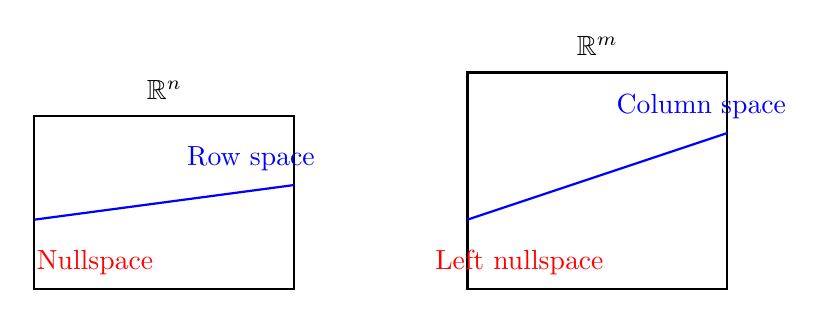
\begin{tikzpicture}[scale=1.1]
% domain R^n
\draw[thick] (0,0) rectangle (3,2);
\node at (1.5,2.3) {$\mathbb{R}^n$};
\draw[thick,blue] (0,0.8) -- (3,1.2);
\node[blue] at (2.5,1.5) {Row space};
\node[red] at (0.7,0.3) {Nullspace};

% codomain R^m
\draw[thick] (5,0) rectangle (8,2.5);
\node at (6.5,2.8) {$\mathbb{R}^m$};
\draw[thick,blue] (5,0.8) -- (8,1.8);
\node[blue] at (7.7,2.1) {Column space};
\node[red] at (5.6,0.3) {Left nullspace};
\end{tikzpicture}
\end{center}

\section*{Własności}
\begin{itemize}
  \item $\dim \mathcal{C}(A)=\dim \mathcal{C}(A^\top)=\mathrm{rank}(A)=r$.
  \item $\dim \mathcal{N}(A)=n-r$, \quad $\dim \mathcal{N}(A^\top)=m-r$.
  \item Każdy $x\in\mathbb{R}^n$ można jednoznacznie zapisać jako
        $x=x_{\mathrm{row}}+x_{\mathrm{null}}$.
  \item Każdy $y\in\mathbb{R}^m$ można jednoznacznie zapisać jako
        $y=y_{\mathrm{col}}+y_{\mathrm{left}}$.
\end{itemize}

\section*{Zadania}
\begin{enumerate}[label=\textbf{Z\arabic*}.]
  \item Dla
  \(
  A=\begin{bmatrix}1&2\\0&0\\0&0\end{bmatrix}
  \)
  wyznacz wszystkie cztery podprzestrzenie. Sprawdź ortogonalność.
  \item Dla
  \(
  A=\begin{bmatrix}1&1&0\\0&1&1\end{bmatrix}
  \)
  znajdź $\mathcal{C}(A),\ \mathcal{N}(A),\ \mathcal{C}(A^\top),\ \mathcal{N}(A^\top)$
  i sprawdź rozkład $\mathbb{R}^3=\mathcal{C}(A^\top)\oplus \mathcal{N}(A)$.
  \item Udowodnij, że LSQ $\min_x\|Ax-b\|$ odpowiada rzutowi $b$ na $\mathcal{C}(A)$.
  \item Sprawdź równości wymiarów:
  \[
  \dim \mathcal{C}(A)+\dim \mathcal{N}(A^\top)=m, \quad
  \dim \mathcal{C}(A^\top)+\dim \mathcal{N}(A)=n.
  \]
  \item \textbf{(Iloczyn skalarny a ortogonalność przestrzeni)}  
  Niech $\langle u,v\rangle = u^\top v$ będzie standardowym iloczynem skalarnym.
  \begin{enumerate}[label=(\alph*)]
    \item Pokaż tożsamość
    \[
      \langle Ax,\,y\rangle \;=\; y^\top A x \;=\; x^\top A^\top y \;=\; \langle x,\,A^\top y\rangle
    \]
    dla dowolnych $x\in\mathbb{R}^n$, $y\in\mathbb{R}^m$.
    \item Wykaż, że
    \[
      \mathcal{N}(A) \;=\; \big(\mathcal{C}(A^\top)\big)^\perp
      \qquad\text{oraz}\qquad
      \mathcal{N}(A^\top) \;=\; \big(\mathcal{C}(A)\big)^\perp.
    \]
    (Wskazówka: użyj punktu (a) z $y$ lub $x$ należącymi do odpowiedniej przestrzeni).
    \item Z (b) wywnioskuj rozkłady ortogonalne
    \[
      \mathbb{R}^n = \mathcal{C}(A^\top)\oplus \mathcal{N}(A),
      \qquad
      \mathbb{R}^m = \mathcal{C}(A)\oplus \mathcal{N}(A^\top).
    \]
    \item \emph{(Połączenie ze SVD)} Niech $A=U\Sigma V^\top$ ma rząd $r$.
    Pokaż, że projekcje ortogonalne na przestrzeń kolumn i wierszy mają postać
    \[
      P_{\mathrm{col}} = U_r U_r^\top,\qquad
      P_{\mathrm{row}} = V_r V_r^\top,
    \]
    gdzie $U_r$ (resp. $V_r$) zbudowane jest z pierwszych $r$ kolumn $U$ (resp. $V$).
    \item \emph{(Krótka weryfikacja numeryczna)} Dla macierzy z \textbf{Z1} lub \textbf{Z2}
    wyznacz $U_r, V_r$ i sprawdź numerycznie, że $P_{\mathrm{col}}^2=P_{\mathrm{col}}$, 
    $P_{\mathrm{row}}^2=P_{\mathrm{row}}$, oraz że $P_{\mathrm{col}}$ rzutuje na $\mathcal{C}(A)$,
    a $P_{\mathrm{row}}$ na $\mathcal{C}(A^\top)$.
    \item \emph{(Bonus – LSQ)} Pokaż, że dla rozwiązania LSQ $x^\star$ reszta
    $r=b-Ax^\star$ należy do $\mathcal{N}(A^\top)$, czyli jest ortogonalna do $\mathcal{C}(A)$.
  \end{enumerate}
\end{enumerate}


\section*{English Corner}
\begin{quote}
\textbf{The four fundamental subspaces:}
\begin{enumerate}
\item Column space of \(A\) – all linear combinations of the columns.
\item Nullspace of \(A\) – all solutions of \(Ax=0\).
\item Row space of \(A\) – column space of \(A^\top\).
\item Left nullspace of \(A\) – all \(y\) with \(A^\top y=0\).
\end{enumerate}

\medskip
\textbf{Task:} Translate into Polish and explain in your own words.
\end{quote}

\end{document}
